%
\documentclass[
  notoc % Suppress Tufte style table of contents.
]{tufte-book}

% Required Tufte packages.
\usepackage{changepage} % or changepage
\usepackage{fancyhdr}
\usepackage{fontenc}
\usepackage{geometry}
\usepackage{hyperref}
\usepackage{natbib}
\usepackage{bibentry}
\usepackage{optparams}
\usepackage{paralist}
\usepackage{placeins}
\usepackage{ragged2e}
\usepackage{setspace}
\usepackage{textcase}
\usepackage{textcomp}
\usepackage{titlesec}
\usepackage{titletoc}
\usepackage{xcolor}
\usepackage{xifthen}

\geometry{paperheight=10in,paperwidth=7in,marginparwidth=30mm,marginparsep=2mm,bindingoffset=10mm,top=10mm,inner=8mm,outer=8mm,bottom=16mm,includehead,includemp}

% Tufte vs. Pandoc workaround.
% Issue: https://github.com/Tufte-LaTeX/tufte-latex/issues/64.
\renewcommand\allcapsspacing[1]{{\addfontfeature{LetterSpace=15}#1}}
\renewcommand\smallcapsspacing[1]{{\addfontfeature{LetterSpace=10}#1}}

% \setmainfont{TeX Gyre Pagella}
\usepackage[utf8]{inputenc}
\usepackage[T1]{fontenc}
\setmainfont{texgyrepagella}[
  Extension = .otf,
  UprightFont = *-regular,
  BoldFont = *-bold,
  ItalicFont = *-italic,
  BoldItalicFont = *-bolditalic,
]

\newfontfamily\JuliaMono{JuliaMono}[
  UprightFont = *-Regular,
  BoldFont = *-Bold
]
\newfontface\JuliaMonoRegular{JuliaMono-Regular}
\newfontface\JuliaMonoBold{JuliaMono-Bold}

\setmonofont{JuliaMono-Medium}[
  Contextuals=Alternate,
  Ligatures=NoCommon
]


\usepackage{graphicx}
\makeatletter
\def\maxwidth{\ifdim\Gin@nat@width>\linewidth\linewidth\else\Gin@nat@width\fi}
\def\maxheight{\ifdim\Gin@nat@height>\textheight\textheight\else\Gin@nat@height\fi}
\makeatother
% Scale images if necessary, so that they will not overflow the page
% margins by default, and it is still possible to overwrite the defaults
% using explicit options in \includegraphics[width, height, ...]{}
\setkeys{Gin}{width=\maxwidth,height=\maxheight,keepaspectratio}
\DeclareRobustCommand{\href}[2]{#2\footnote{\url{#1}}}

\usepackage{float}
\floatplacement{figure}{H}

% Listings Julia syntax definition.
\input{/home/runner/.julia/packages/Books/C7CMR/defaults/julia_listings.tex}

% Unicode support.
\input{/home/runner/.julia/packages/Books/C7CMR/defaults/julia_listings_unicode.tex}

% Used by Pandoc.
\providecommand{\tightlist}{%
  \setlength{\itemsep}{0pt}\setlength{\parskip}{0pt}
}
\newcommand{\passthrough}[1]{#1}

\usepackage{longtable}
\usepackage{booktabs}
\usepackage{array}

% Source: Wandmalfarbe/pandoc-latex-template.
\newlength{\cslhangindent}
\setlength{\cslhangindent}{1.5em}
\newlength{\csllabelwidth}
\setlength{\csllabelwidth}{3em}
\newenvironment{CSLReferences}[2] % #1 hanging-ident, #2 entry spacing
 {% don't indent paragraphs
  \setlength{\parindent}{0pt}
  % turn on hanging indent if param 1 is 1
  \ifodd #1 \everypar{\setlength{\hangindent}{\cslhangindent}}\ignorespaces\fi
  % set entry spacing
  \ifnum #2 > 0
  \setlength{\parskip}{#2\baselineskip}
  \fi
 }%
 {}
\usepackage{calc}
\newcommand{\CSLBlock}[1]{#1\hfill\break}
\newcommand{\CSLLeftMargin}[1]{\parbox[t]{\csllabelwidth}{#1}}
\newcommand{\CSLRightInline}[1]{\parbox[t]{\linewidth - \csllabelwidth}{#1}\break}
\newcommand{\CSLIndent}[1]{\hspace{\cslhangindent}#1}

\definecolor{linkblue}{HTML}{117af2}
\usepackage{hyperref}
\hypersetup{
  colorlinks,
  citecolor=linkblue,
  linkcolor=linkblue,
  urlcolor=linkblue,
  linktoc=page, % Avoid Table of Contents being nearly completely blue.
  pdftitle={Bayesian assignment},
  pdfauthor={Rik Huijzer; Don van Ravenzwaaij},
  pdflang={en-US},
  breaklinks=true,
  pdfcreator={LaTeX via Pandoc}%
}
\urlstyle{same} % disable monospaced font for URLs

\title{Bayesian assignment}
\author{\noindent{Rik Huijzer}\\[3mm] \noindent{Don van
Ravenzwaaij}\\[3mm] }
\date{}

% Re-enable section numbering which was disabled by tufte.
\setcounter{secnumdepth}{2}

% Fix captions for longtable.
% Thanks to David Carlisle at https://tex.stackexchange.com/a/183344/92217.
\makeatletter
\def\LT@makecaption#1#2#3{%
  \noalign{\smash{\hbox{\kern\textwidth\rlap{\kern\marginparsep
  \parbox[t]{\marginparwidth}{\vspace{12pt}%
\@tufte@caption@font \@tufte@caption@justification \noindent
   #1{#2: }\ignorespaces #3}}}}}}
\makeatother

% Doesn't seem to do anything.
\usepackage{float}
\floatplacement{figure}{H}
\floatplacement{table}{H}

% Reduce large spacing around sections.
\titlespacing*{\chapter}{0pt}{5pt}{20pt}
\titlespacing*{\section}{0pt}{2.5ex plus 1ex minus .2ex}{1.3ex plus .2ex}
\titlespacing*{\subsection}{0pt}{1.75ex plus 1ex minus .2ex}{1.0ex plus.2ex}

\titleformat{\chapter}%
  [hang]% shape
  {\normalfont\huge\itshape}% format applied to label+text
  {\huge\thechapter}% label
  {1em}% horizontal separation between label and title body
  {}% before the title body
  []% after the title body

% Reduce spacing in table of contents.
\usepackage{etoolbox}
\makeatletter
\pretocmd{\chapter}{\addtocontents{toc}{\protect\addvspace{-3\p@}}}{}{}
\pretocmd{\section}{\addtocontents{toc}{\protect\addvspace{-4\p@}}}{}{}
\pretocmd{\subsection}{\addtocontents{toc}{\protect\addvspace{-5\p@}}}{}{}
\makeatother

% Long texts are harder to read than tables.
% Therefore, we can reduce the font size of the table.
\AtBeginEnvironment{longtable}{\footnotesize}

% Some space between paragraphs is necessary because code blocks can output single line paragraphs.
\setlength\parskip{1em plus 0.1em minus 0.2em}

% For justified text.
\usepackage{ragged2e}

% tufte-book disables subsubsections by default.
% Got this definition back via `\show\subsubsection`.

\usepackage{amsfonts}
\usepackage{amssymb}
\usepackage{amsmath}
\usepackage{unicode-math}

% URL line breaks.
\usepackage{xurl}

% Probably doesn't hurt.
\usepackage{marginfix}

\let\cleardoublepage\clearpage

\begin{document}

\makeatletter
\thispagestyle{empty}
\vfill
{\Huge\bf
\noindent
\@title
}\\[1in]
{\Large
\noindent
\@author
}
\makeatother

\makeatletter
\newpage
\thispagestyle{empty}
\vfill
{\noindent
\begin{tabular}{l}
Rik Huijzer \\
Don van Ravenzwaaij \\
\\
University of Groningen
\end{tabular}
}
\vfill
{\small
\url{https://rikhuijzer.github.io/BayesianAssignment.jl/}

2022-10-15

Creative Commons Attribution-NonCommercial-ShareAlike 4.0 International
}
\makeatother


% Don't remove this or authors will show up in header of every page.
\frontmatter
\mainmatter

\setcounter{tocdepth}{1}
\tableofcontents

% Justify text.
\justifying

% parindent seems to be set from within another class too.
% it is really not useful here because it will also indent lines directly after
% code blocks. Which most of the times not useful.
\setlength{\parindent}{0pt}

\hypertarget{sec:background}{%
\chapter{Background}\label{sec:background}}

Throughout the course of your psychology cirriculum, you have been
exposed to Null Hypothesis Significance Testing (NHST) on numerous
occasions. NHST is arguably the golden standard in inferential
statistics in psychology, but it does not come without its shortcomings.
In this course, we are going to focus on one specific issue: the
inability to find evidence \emph{in favor} of the null hypothesis.

There are a lot of reasons why one might want to quantify evidence in
favor of the null. For one, some fields in psychology are in a ``crisis
of confidence'' (see e.g.,
\protect\hyperlink{ref-pashler2012editors}{Pashler \& Wagenmakers,
2012}). In this crisis, many claims have been made, with statistical
support, which turn out not to be true. One way to undo these results is
to gather statistical evidence against these false claims.

In this module, you are presented with an alternative inferential
framework: Bayesian statistics. In the first lecture, you will learn
about the philosophy behind Bayesian statistics, how it conceptually
works, and its advantages and disadvantages compared to conventional
inferential statistics. In the second lecture, you will be introduced to
a synthetic dataset from Rik's research. With this dataset, you will be
able to obtain roughly the same results as Rik and the co-authors got.
The assignment in this module asks you to analyze this dataset yourself.
You will conduct both conventional and Bayesian inference and write a
results section that showcases your findings. You will not only report
that an effect is there, but also that an effect is \textbf{not} there.

\hypertarget{sec:assignment}{%
\chapter{Assignment}\label{sec:assignment}}

In this assignment, we will look into the differences in the Big Five
personality traits of Dutch special operations forces (henceforth,
commandos) versus the general population. Commandos are elite military
troops, so they are required to perform well in extreme mental and
physical conditions. Therefore, we expect that commandos are less
neurotic (sensitive/nervous) than civilians
(\protect\hyperlink{ref-jackson2012military}{Jackson et al., 2012};
\protect\hyperlink{ref-lee2011prospective}{Lee et al., 2011};
\protect\hyperlink{ref-mcdonald1990training}{McDonald et al., 1990}).
Also, we expect that commandos are more extravert (outgoing/energetic)
than civilians (\protect\hyperlink{ref-jackson2012military}{Jackson et
al., 2012}).

The synthetic data provided with this assignment consists of the
personality scores of commandos and civilians on neuroticism (N) and
extraversion (E). The first and last few rows of the dataset are shown
in Table~\ref{tbl:dataset}.

\hypertarget{tbl:dataset}{}
\begin{longtable}[]{@{}rrrr@{}}
\caption{\label{tbl:dataset}First and last few rows of the
dataset.}\tabularnewline
\toprule
participant & group & neuroticism & extraversion \\
\midrule
\endfirsthead
\toprule
participant & group & neuroticism & extraversion \\
\midrule
\endhead
1 & commandos & 103.01 & 154.78 \\
2 & commandos & missing & 162.86 \\
3 & commandos & 124.47 & 171.24 \\
4 & commandos & 97.81 & missing \\
\ldots{} & \ldots{} & \ldots{} & \ldots{} \\
382 & civilians & 131.84 & 158.24 \\
383 & civilians & 87.12 & 118.44 \\
384 & civilians & missing & 159.1 \\
385 & civilians & 138.48 & 164.14 \\
\bottomrule
\end{longtable}

You can download the data via:\\
\url{https://rikhuijzer.github.io/BayesianAssignment.jl/data.csv}

To give you a bit of an intuition about this dataset, we visualize it by
plotting all the points, see Figure~\ref{fig:not_so_useful}. This figure
is a bit misleading since there could be many points lying on top of
each other.

\begin{figure}
\hypertarget{fig:not_so_useful}{%
\centering
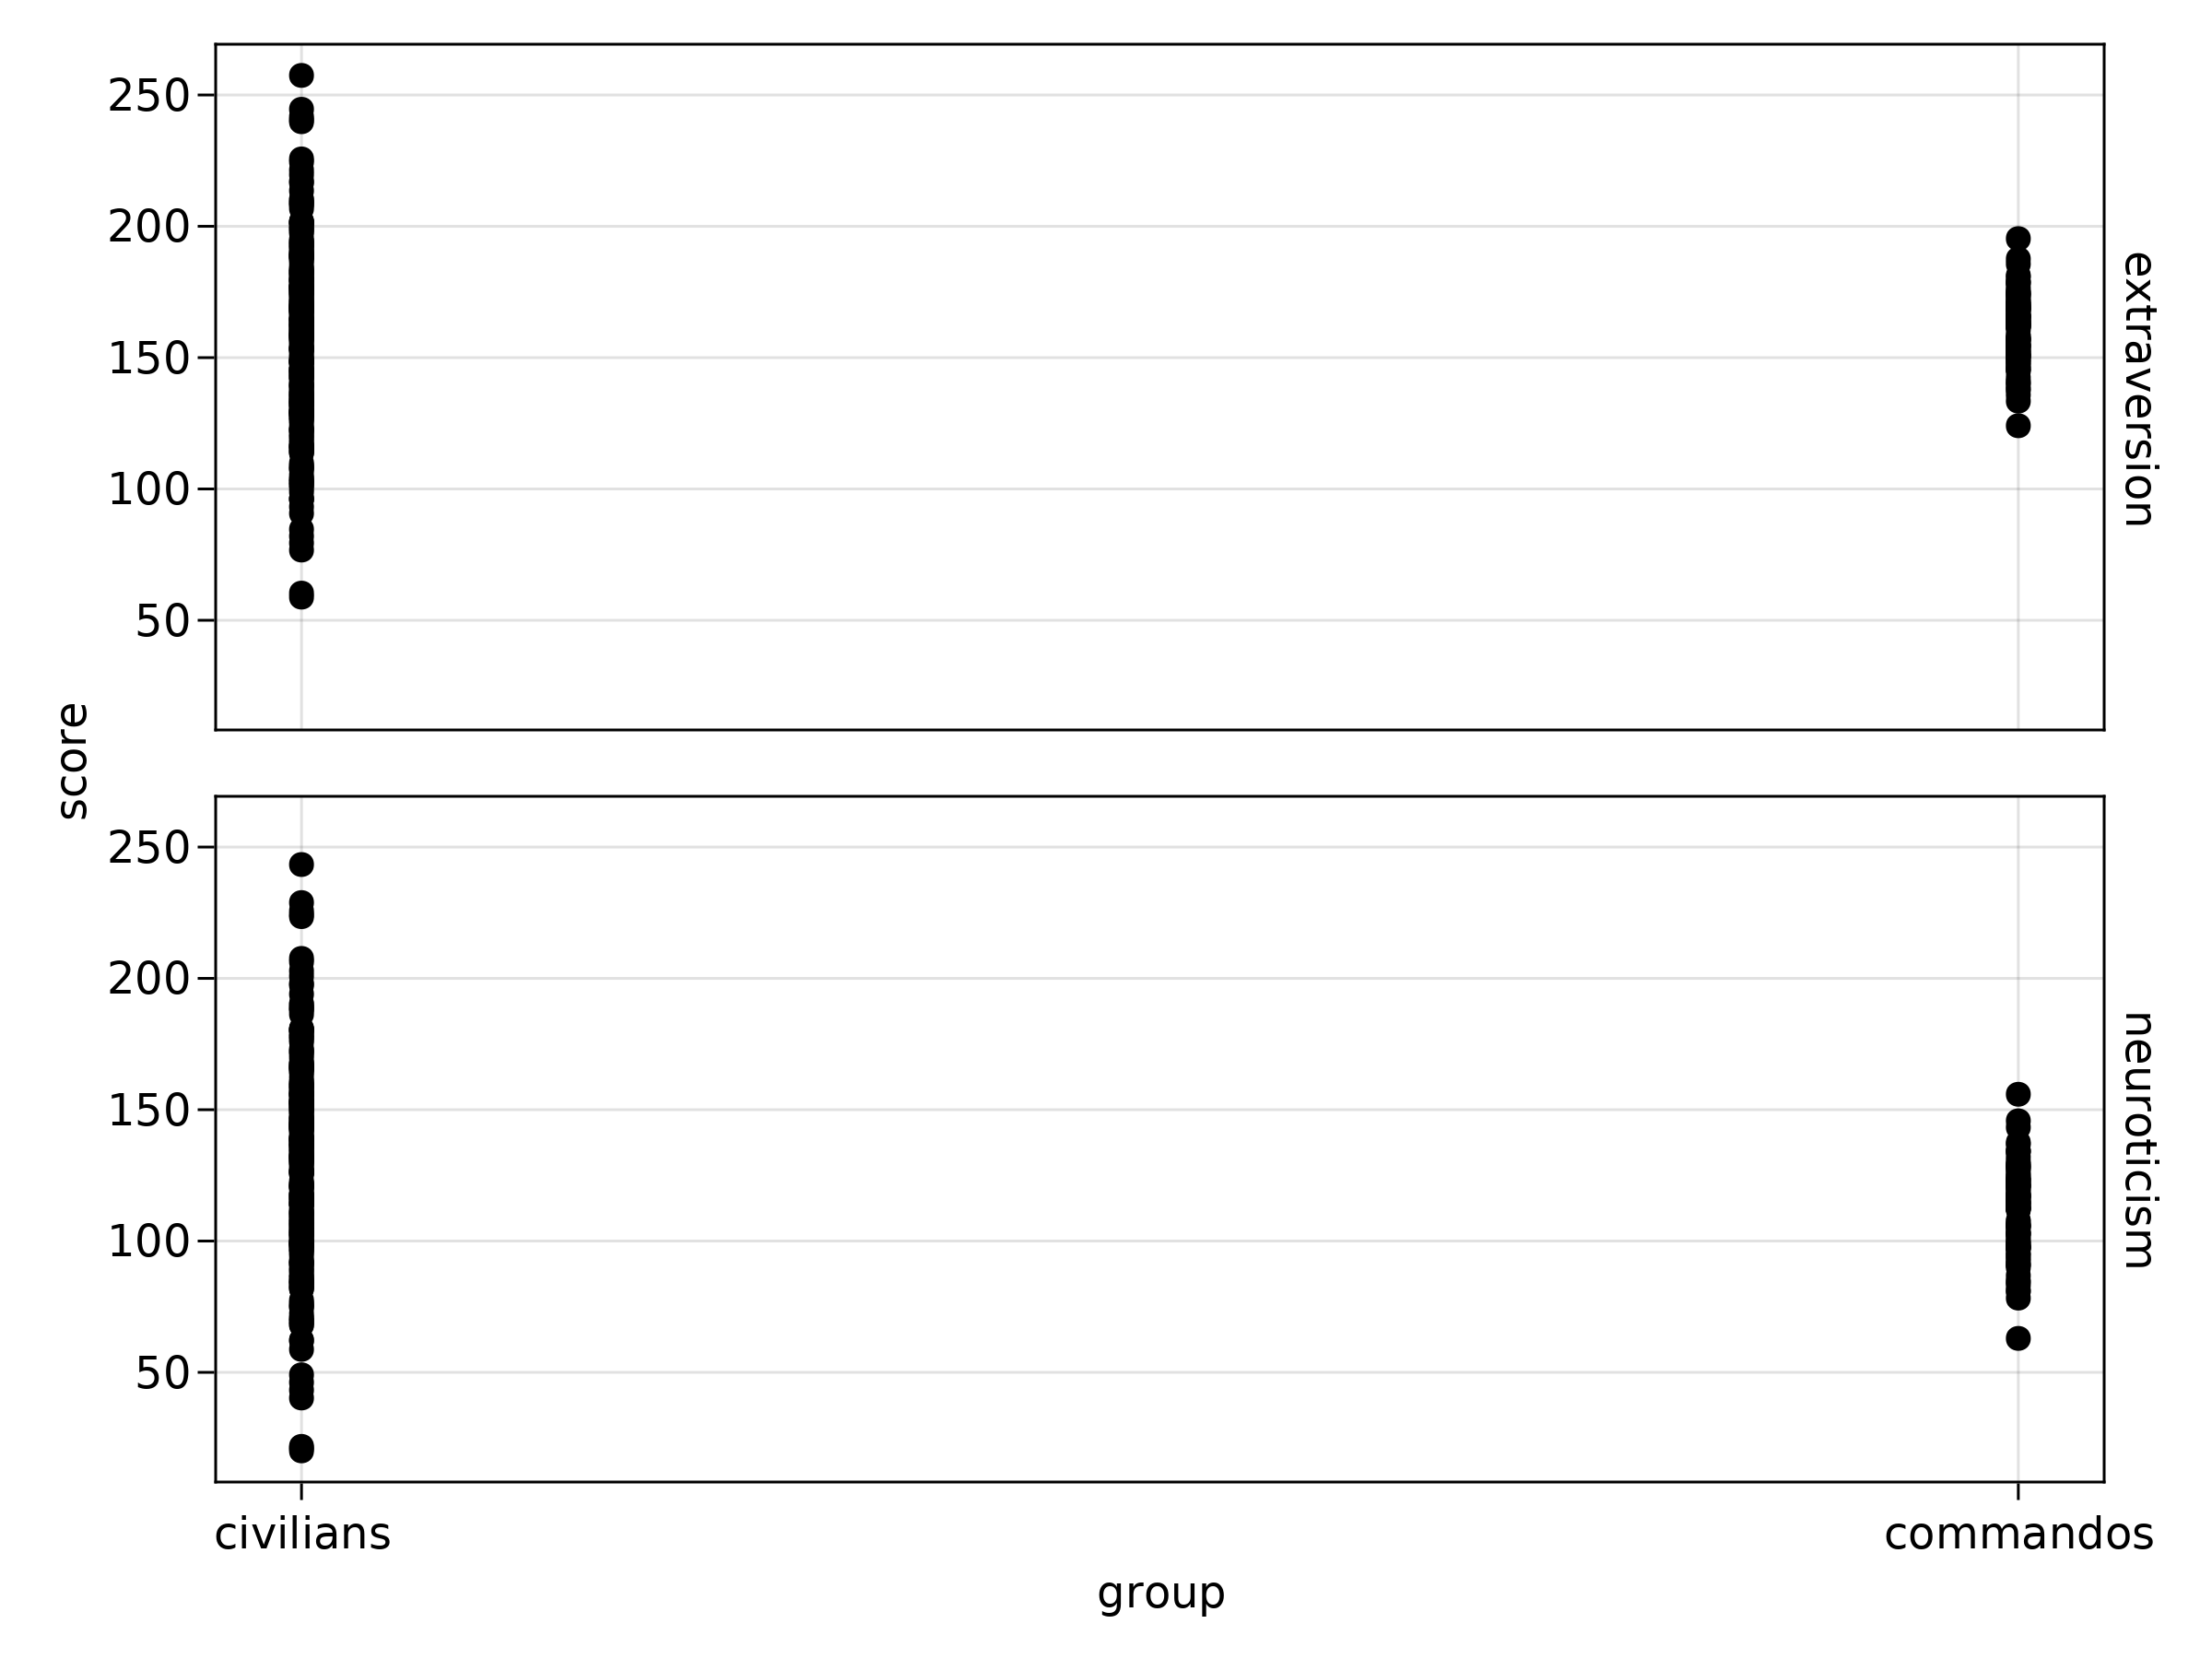
\includegraphics{_build/im/let_fg_BayesianAssignment_plot_points_caption_A_simple_but_possib.png}
\caption{A simple but possibly misleading visualization of the
data.}\label{fig:not_so_useful}
}
\end{figure}

So, instead, we can also visualize it by estimating the distribution via
a, so called, kernel density estimator (Figure~\ref{fig:kde}).
(Basically, this means: throw all the scores on different piles and make
it prettier by smoothing it all out a bit. Understanding this is not
required for the assignment.)

\begin{figure}
\hypertarget{fig:kde}{%
\centering
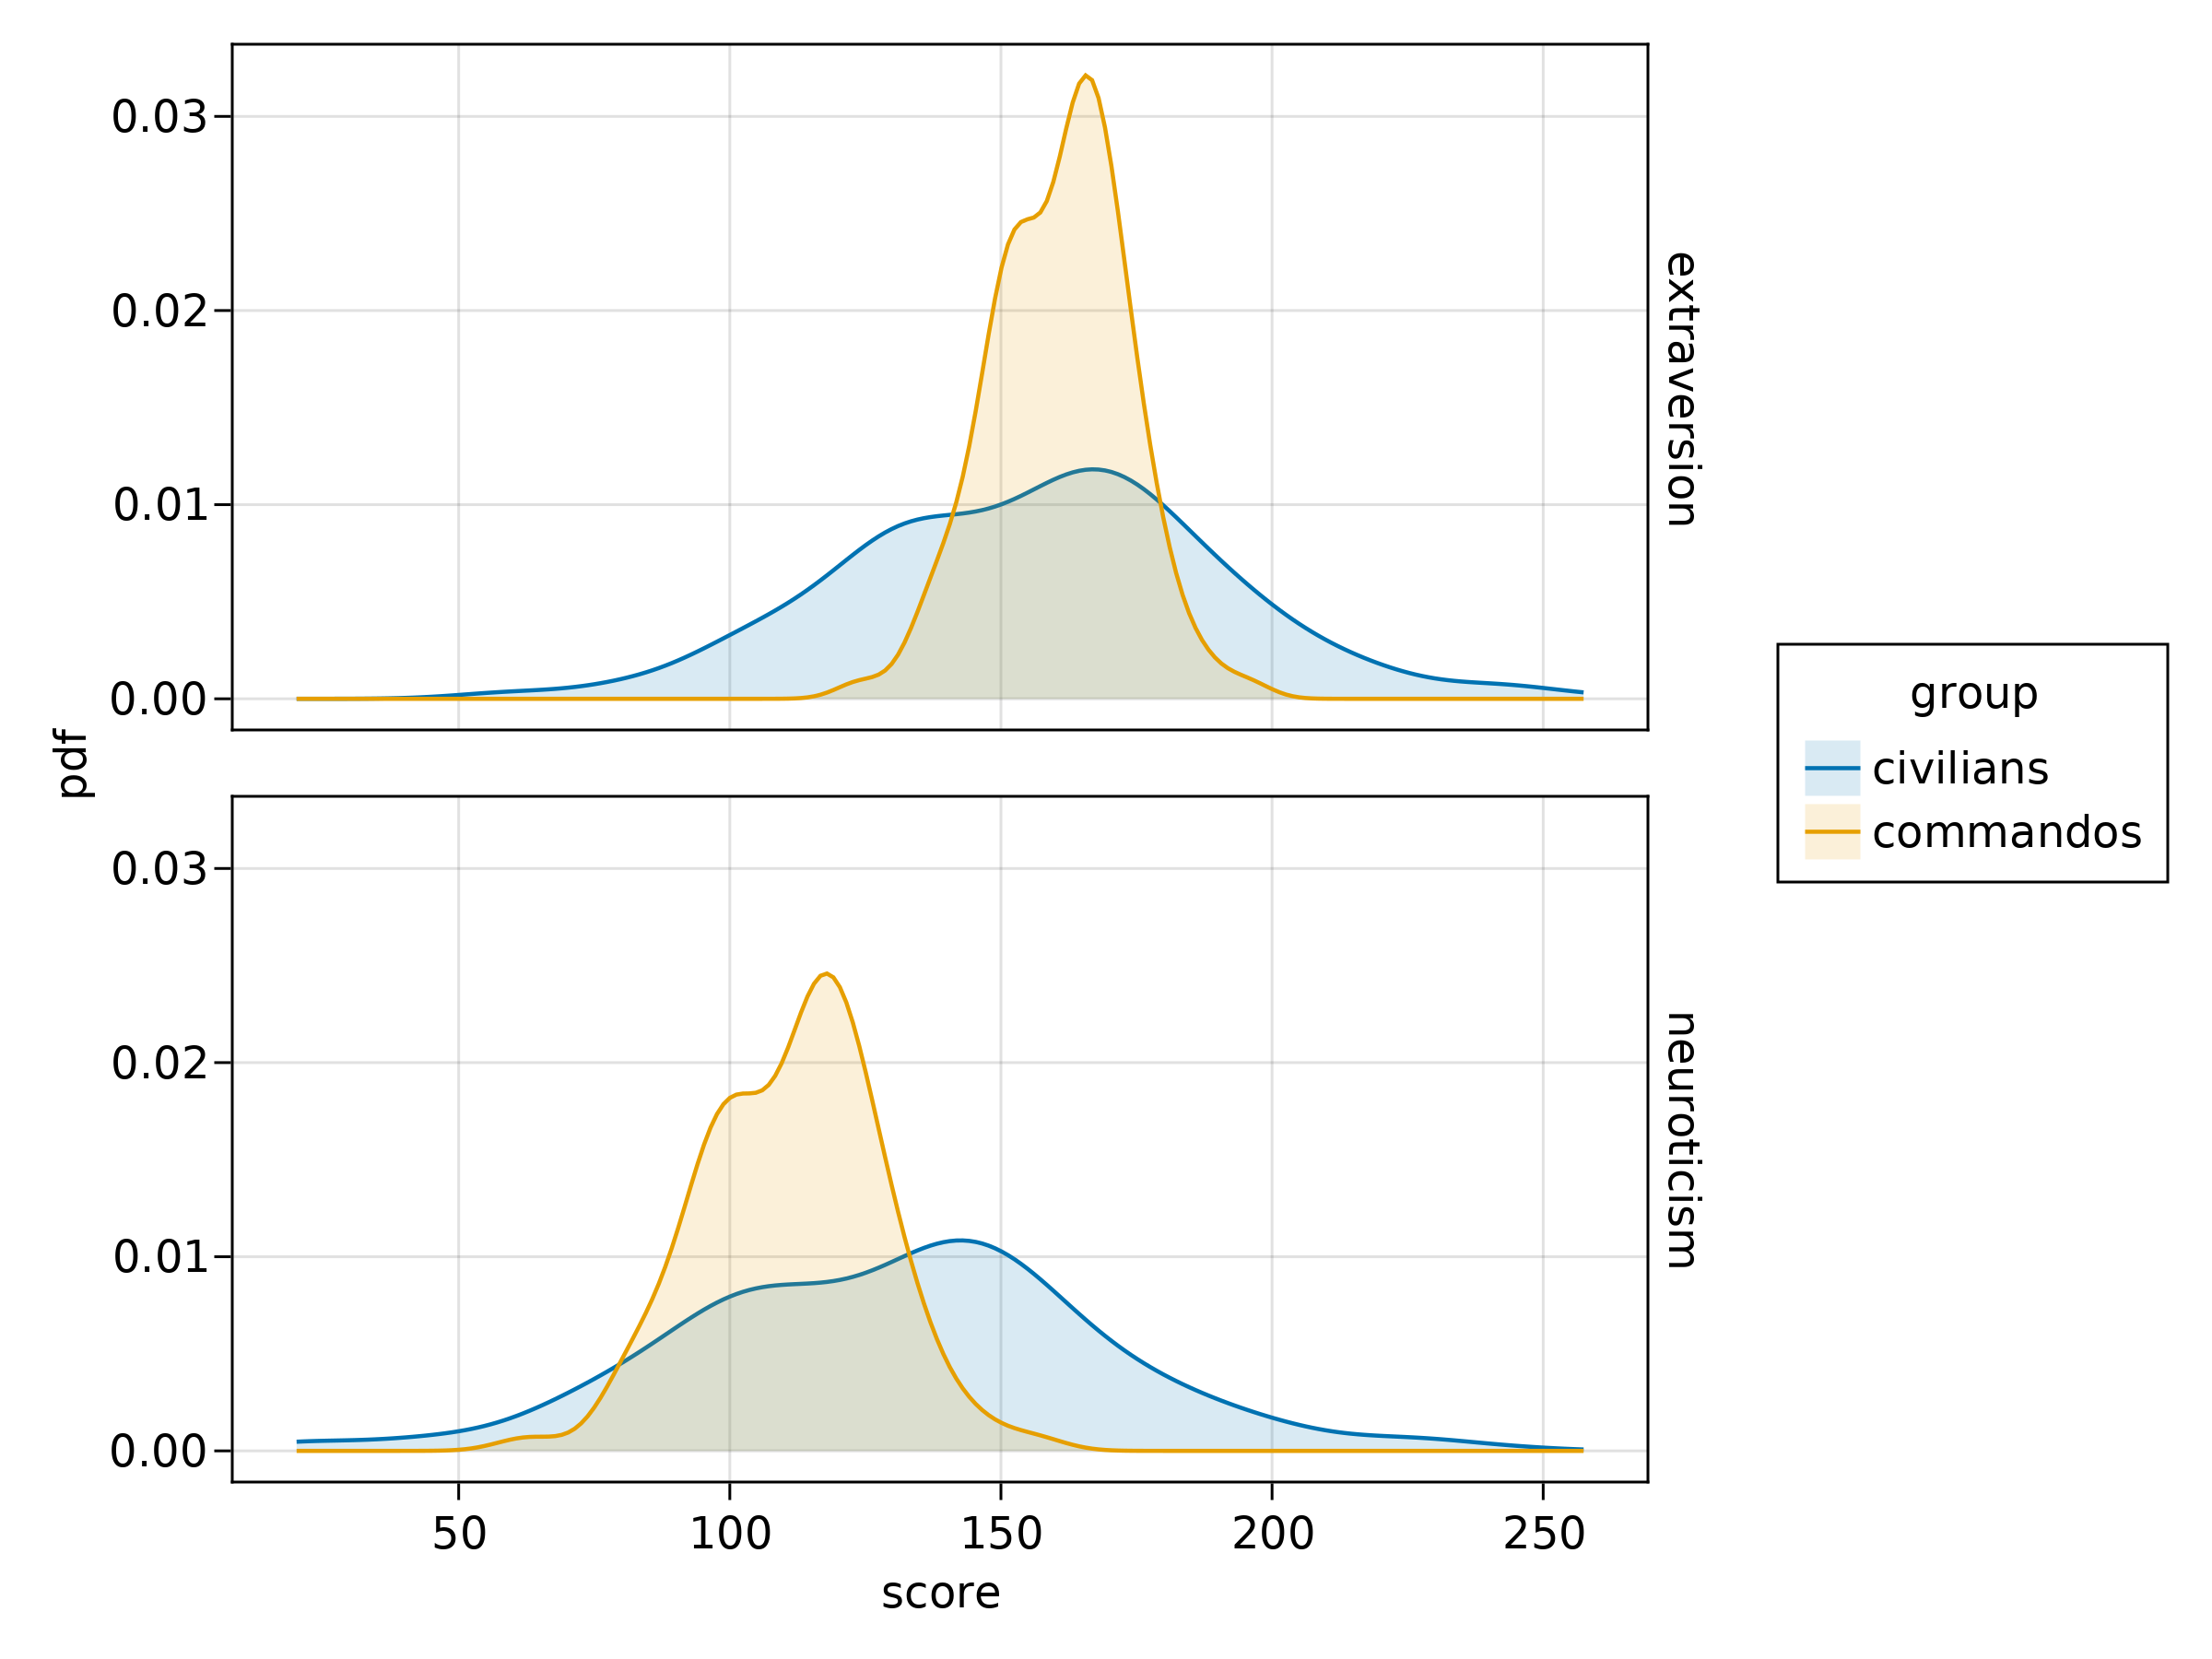
\includegraphics{_build/im/fg_BayesianAssignment_plot_density_caption_Estimation_of_the_distribution.png}
\caption{Estimation of the distributions.}\label{fig:kde}
}
\end{figure}

\newpage

\begin{enumerate}
\def\labelenumi{\arabic{enumi}.}
\item
  \emph{{[}2 pt{]}} The data contains many missing values. Clean up the
  data by using the pass-through filter in JASP. Report what formula you
  use in the filter and how many rows remain. Note that, to apply
  multiple filters at the same time, you can use something like
  \((\text{neuroticism} \cdots ) \land ( \cdots )\).
\item
  \emph{{[}2 pt{]}} Create boxplots for neuroticism and extraversion
  while also splitting the data up in groups. Add the plots to your
  report.
\item
  \emph{{[}3 pt{]}} Report results for doing traditional inference
  tests. Think about the design, report what test you are using. Is it a
  \emph{t}-test (if yes, one- or two-tailed?), an ANOVA (if yes, what
  contrasts, post-hoc tests?), a linear regression, or something else?
  Report your test statistic, the degrees of freedom, and the obtained
  p-value.
\item
  \emph{{[}3 pt{]}} Report results for Bayesian inference. Make sure you
  use the same kind of analysis as you did for the traditional approach
  (you will find the Bayesian equivalent under the same button). Report
  the Bayes factor and include a plot of the sequential Bayes factor
  (tick the box that says ``Sequential analysis'').
\end{enumerate}

\hypertarget{references}{%
\chapter*{References}\label{references}}
\addcontentsline{toc}{chapter}{References}

\hypertarget{refs}{}
\begin{CSLReferences}{1}{0}
\leavevmode\hypertarget{ref-jackson2012military}{}%
Jackson, J. J., Thoemmes, F., Jonkmann, K., Lüdtke, O., \& Trautwein, U.
(2012). Military training and personality trait development: Does the
military make the man, or does the man make the military?
\emph{Psychological Science}, \emph{23}(3), 270--277.
\url{https://doi.org/10.1177/0956797611423545}

\leavevmode\hypertarget{ref-lee2011prospective}{}%
Lee, J. E. C., McCreary, D. R., \& Villeneuve, M. (2011). {Prospective
multifactorial analysis of Canadian Forces basic training attrition}.
\emph{Military Medicine}, \emph{176}(7), 777--784.
\url{https://doi.org/10.7205/MILMED-D-10-00375}

\leavevmode\hypertarget{ref-mcdonald1990training}{}%
McDonald, D. G., Norton, J. P., \& Hodgdon, J. A. (1990). {Training
success in U.S. Navy special forces.} \emph{Aviation, Space, and
Environmental Medicine}.

\leavevmode\hypertarget{ref-pashler2012editors}{}%
Pashler, H., \& Wagenmakers, E. (2012). Editors' introduction to the
special section on replicability in psychological science: A crisis of
confidence? \emph{Perspectives on Psychological Science}, \emph{7}(6),
528--530. \url{https://doi.org/10.1177/1745691612465253}

\end{CSLReferences}

\backmatter

\end{document}
